\chapter{Introduction}
\label{introduction0}
\vspace{-0.25cm}
\section{The Complexity Conundrum}
\label{introduction1}

\begin{flushright}
\textit{``Reality is 80 million polygons per second''\,\footnote{ \textit{``There used to be this quipped saying back in the early days of 3D rendering. It was a great catchphrase at the time because during those days, it was an obscene number -- ridiculously beyond the technology of the day. But nowadays, ... , even cheap console systems can crank out that kind of performance. More importantly, today's technology can render that many polygons in realtime with tons more features than was ever available before, such as programmability or multiple passes. And the high-end keeps getting higher.''} \citep[John Carmack, co-founder of id Software, on that very quote, cited in:][]{Kosak2005}}}\\
-- Alvey Ray Smith \citep[co-founder Pixar, cited in:][p.168]{Rheingold1991}
\end{flushright}

Computer Graphics, much as related fields in Computer Science, has seen an awe-inspiring rate of progress over the last decades.
Yet it seems to be a peculiar fact that advances in Computer Graphics at times appear to be invisible, albeit being often directly translated to prettier pictures and more visceral applications.\\
Normally at this point most people reference the infamous success story of increased computational power, known as \textit{Moore’s Law}\footnote{ The prediction was initially stated in 1965 by Intel co-founder Gordon Moore and held up with physical law-like precision for the last half-century (for the original reference and its context see Appendix \ref{appendix1}).}.
Less widely understood, but even more remarkable is the fact that in most areas, performance gains due to improvements in algorithms have vastly exceeded the performance gains due to increased processor speed\footnote{ It’s difficult to quantify the improvement, though, because it is as much in the realm of quality as of execution time.
In the field of numerical algorithms, however, the improvements can be quantified more straightforwardly.
One example, provided by Prof. Martin Grötschel: A benchmark production planning model solved using linear programming improved by a factor of roughly 43 million between 1991 and 2008.
Of this, a factor of roughly 1,000 was due to increased processor speed, whereas a factor of roughly 43,000 was due to improvements in algorithms \citep[][cf. p.71]{Holdren2010}.}.
When asked about the significant advances over the last 20 years \textit{Ed Catmull} explained how sometimes \textit{``we felt it was at an impossible level''} what they were trying to reach in terms of quality, but now years later \textit{``we have exceeded that level in terms of scene and render complexity -- we have gone beyond impossible''}\,\footnote{ See Appendix \ref{appendix2} for a timeline of important technological advances of RednerMan\textsuperscript{\textregistered}.} \citep[Edwin „Ed“ Catmull, president of Walt Disney \& Pixar Animation Studios, citet in:][]{Seymour2008}.\\
Despite the industries incredible success, \textit{Catmulls} remark about the complexity as being \textit{“beyond impossible”} appears to contradict the notion of super-exponential technology growth in the field of Computer Graphics.
For instance, rendering times have been constant\footnote{ For Industrial Light \& Magic’s visual effects work on the 1993 film Jurassic Park, typical overnight render times were 4 hours per frame. When the same company worked on the 1997 movie sequel, using both faster computers and more advanced software, frame times were typically an identical 4 hours. Each small speed-up, tends to be used for greater input complexity rather than greater interactivity.\\ While the precise value of the “threshold of pain” for render time varies by institution, this effect has been widely observed. Jim Blinn famously remarked, “All frames take 45 minutes,” hence the effect is known as Blinn’s Law \citep[][cf. Chapter 3]{Enderton2011}.}  for animation films over the last two decades, although algorithms and hardware got so much better during the same time.
If the movie business holds as an example\footnote{ Personally, I think that animation and special effects driven movies are vibrant examples for the tremendous progress, that the field of Computer Graphics has seen over the last decades. Although I am sure, other interesting references can be made, most of the examples I will give are related to the \textit{VFX-Industry}. For one because I find them to be compelling and vivid, but more so because it is the one field I have personal experience in, due to my internship at \textit{Weta Digital} in 2011.}, it begs the question: How is this possible?
% Bild
\begin{figure}[ht]
\begin{minipage}[b]{0.475\linewidth} \centering
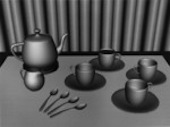
\includegraphics[scale=1.0]{utah_teapot_render.jpg}
\caption{Teapot rendering scene as presented in \textit{Martin Newell's} PhD dissertation, published in 1975 \citep[cf.][]{Torrence2006}.}
\label{fig:utah_teapot_render}
\end{minipage}
\hspace{0.35cm}
\begin{minipage}[b]{0.475\linewidth}
\centering
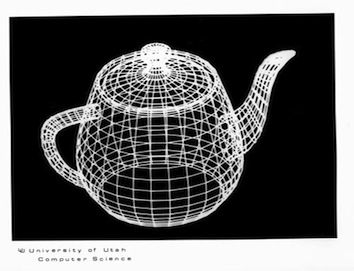
\includegraphics[scale=1.0]{utah_teapot_model.jpg}
\caption{The original wireframe 'Utah Teapot' (28 bicubic Bézier patches, with 16 control points each) \citep[cf.][]{Newell1975a}.}
\label{fig:utah_teapot_model}
\end{minipage}
\end{figure}\\
The answer is ever increasing complexity!
Increasing complexity regarding: Lighting techniques, phenomena that are simulated, and many other domains but most importantly the increased complexity of the assets used for rendering.
Every studio struggles with heavier and heavier assets, i.e. the sheer size in geometry information used for models:
\textit{``Our typical rendered scenes [for work on Marvels 'The Avengers' (2012)] contain over 140 million triangles across thousands of objects though we have pushed over 1 billion polygons''} \citep[Votch Levi, CTO Whiskytree, cited in:][]{Seymour2012}.

To illustrate this hasty evolution, one simply has to look at the stark contrast between the models used for the top-of-the-line renderings of 1975, namely the 'Teapot scene' and a scene from the 2009 movie 'UP', as shown in the pictures \ref{fig:utah_teapot_model} and \ref{fig:micropolys}.
Whereas all the information needed to describe the models in the 'Teapot scene' could be literally fit on one page of paper\footnote{  For more information about the original Teapot renderings and a facsimile of the model description, see Appendix \ref{appendix3}.}, the models currently in production regularly max out in the domain of several giga-bytes of raw data per asset.
% Bild
\begin{figure}[ht]
\begin{minipage}[b]{0.475\linewidth} \centering

\includegraphics[scale=0.72]{screenshot_up.jpg}
\caption{Example of highly detailed surface -- note that the houndstooth pattern of the jacket is genuine geometric data {[}Credit: Pixar 2009{]}.}
\label{fig:screenshot_up}
\end{minipage}
\hspace{0.35cm}
\begin{minipage}[b]{0.475\linewidth}
\centering
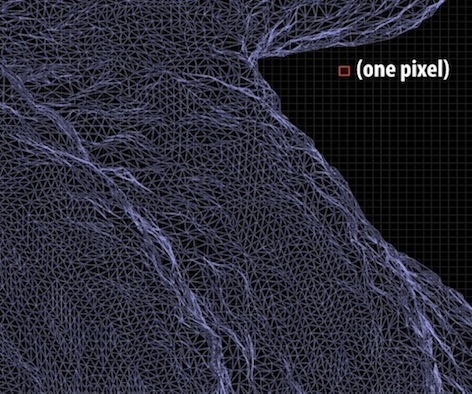
\includegraphics[scale=0.72]{micropolys.jpg}
\caption{To leave no evidence that surfaces are discretely approximated, film models consist of micropolygons, about a pixel in area \citep[][p.7]{Fatahalian2011}.}
\label{fig:micropolys}
\end{minipage}
\end{figure}

\section{The Case for Highly Detailed Geometry}
\label{introduction2}

Regardless of the factual costs and critical handling issues when working with this kind of scope and complexity, the trend appears to be unbroken\footnote{ 
The importance of highly accurate modeled surfaces has always been an crucial factor for (offline) rendering systems \citep[cf.][]{Cook1987}, but especially with tent-pole movie productions, this paradigm seems to know only one direction -- that is -- bigger meshes: ``the complexity continues to scale on each project we do, the amount we need to render continues to multiply...'' -- 'Avatar' (2009), was the first movie project that exceed 2 petabyte of storage data \citep[Martin Hill, head of shading at Weta Digital, cited in:][]{NVidia2009}.}.
The reason for this is, that in order to render richly detailed and artifact-free scenes, complex models are inevitable.
Over the time there have been numerous ingenious strategies to cut corners, such as precomputed static illumination, bump-, normal- and occlusion-mapping, etc. to compensate for the lack of geometric detail, especially in interactive applications \citep[cf.][]{Akenine-Moller2008}.
These techniques have comparatively low rendering cost and are used effectively in games.
However, they are prone to artifacts.
%Bild
\begin{figure}[ht]
\centering
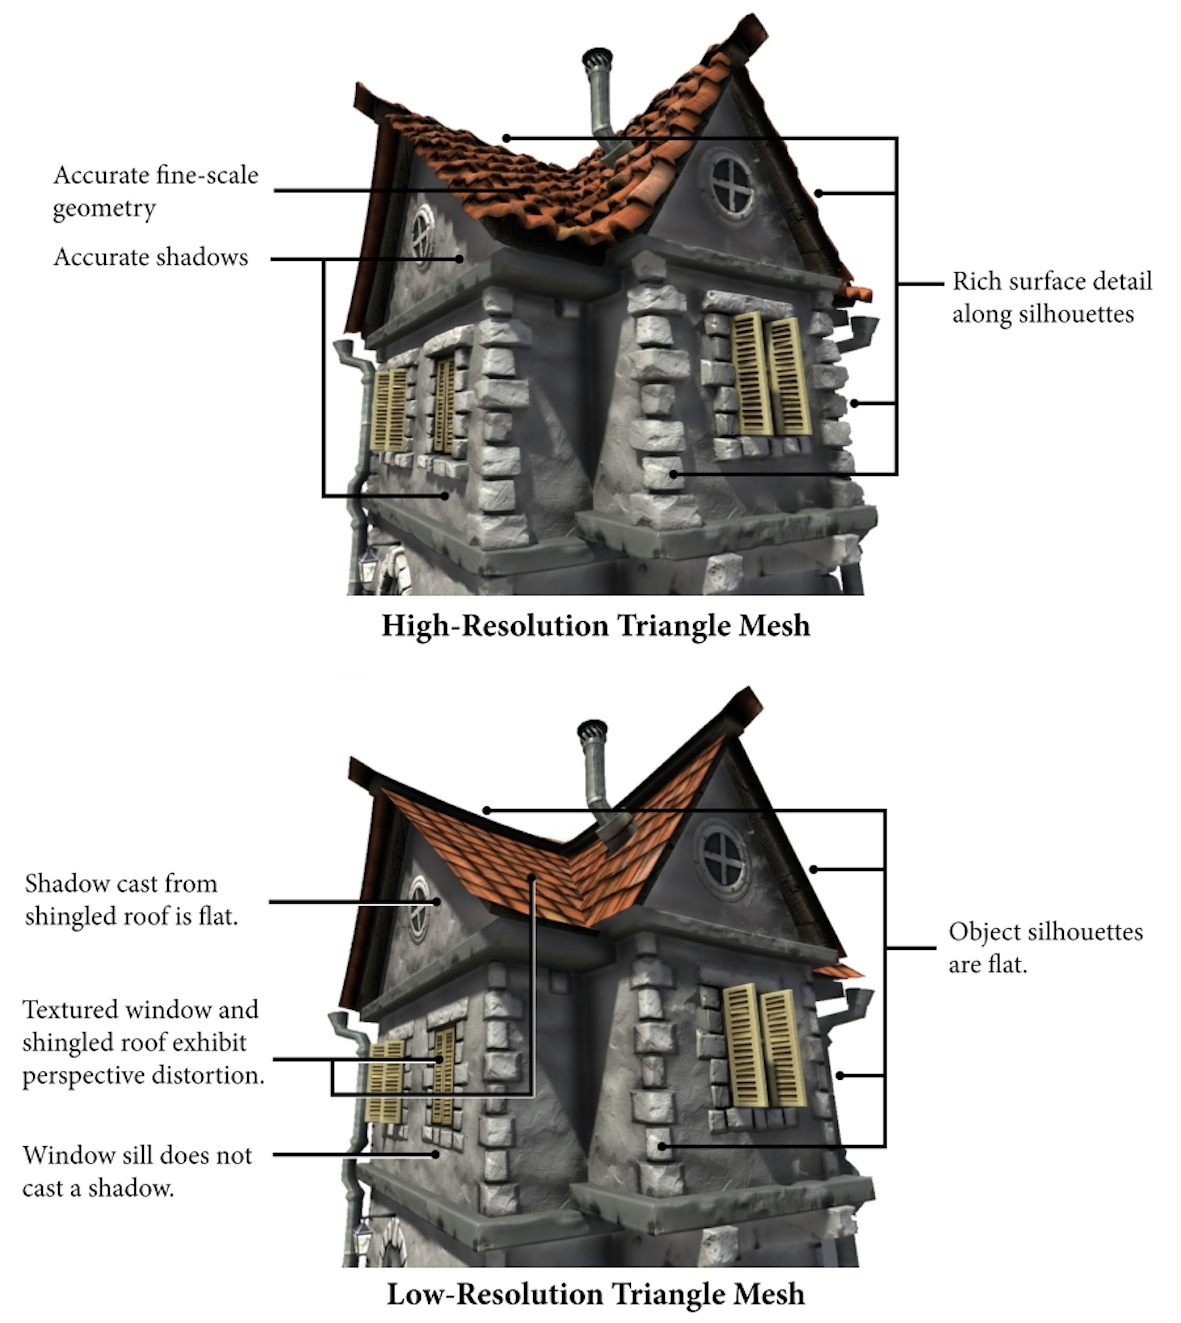
\includegraphics[width=0.95\textwidth]{lowpoly_vs_highpoly.jpg}
\caption{Renderings of a stone house using a high-resolution (top) and low-resolution (bottom) triangle mesh (house image by Unigine Engine).}
\label{fig:lowpoly_vs_highpoly}
\end{figure}\\
The stone house pictured in \ref{fig:lowpoly_vs_highpoly} features many complex surfaces like bumpy cornerstones and curved red roof-tiles.
Accurate shadows (self-shadowing) are cast and self occlusion can be seen.
These details can be rendered because the house is represented using a high-resolution triangle mesh.
The lower image, uses the same texturing and soft shadowing techniques, but with scene geometry represented using a low resolution triangle mesh.
The model holds up quite well, but unfortunately, the illusion breaks down eventually.
Especially along the house’s silhouettes, artifacts are spotted easily.
Shadows are rendered but on close examination they also give away the flat nature of the low resolution stand-in.
Similarly, the roof tiles and windows on the left side of the image appear distorted.
These artifacts become even more noticeable when objects move \citep[cf.][p.2-4]{Fatahalian2011}.\\
The industry will not cease its pursuit for visual brilliance and together with the growing trend for more physically correct rendering, the polygon counts will be constantly pushed for the next years to come.
With this scaling of complexity also scales the need for tools that facilitate the work with the created data\footnote{ During my internship I personally asked a modeler, at what point they would normally stop adding geometric detail. He noted that everyones biggest fear is to get ones' work rejected because it does not hold up to a supervisors expectations. So what they typically will do is to work until their tools -- their computers and software -- give in and make it unbearable to work any further.}.
Thus robust and capable techniques are essential and at the forefront of fundamental techniques for geometry processing is mesh simplification.

\section{Reducing Complexity}
\label{introduction3}

Mesh decimation or simplification is both, a very current, and a very old idea in computer graphics.
As early as 1976 \textit{James Clark} described the benefits of representing objects within a scene at several resolutions \citep[cf.][]{Clark1976}.\\
Dozens and dozens of simplification algorithms have been developed in the meantime.
Even a number of excellent surveys reviewing the field of polygonal simplification have been published\footnote{ For example, Cignoni et al. supplied comparative performance statistics for over 30 different decimation strategies \citep[cf.][]{Cignoni1998, Heckbert1997}.}.
Yet, no algorithm today excels at simplifying all models equally good.
Some approaches best suit curved organic forms, while others work best at preserving hard planar objects with sharp corners, flat faces, and regular curves.
This is probably due to the fact that, we still have limited understanding about what really determines perceptual fidelity.
We do have a good understand of geometric and volumetric fidelity but as it turns out, the supposedly easy question:  Does the simplification look good?
Is hard to answer \citep[][cf. p.25]{Luebke2001}.\\
At this point it seems that the research community tends to be of the opinion, that until the question of perceptual metrics is solved, the research area of mesh simplification is in a state of arrested development\footnote{ Only few ameliorations have been proposed, mostly at the cost of near to prohibitively expense execution times, like Cohen’s ``Appearance-Preserving Simplification'' \citep[cf.][]{Cohen1998} and Lindstrom’s ``Image-Driven Simplification'' \citep[cf.][]{Lindstrom2000} -- both of which aiming at per-pixel comparisons of multiple rendered views as ``weights'' or upper bounds for the priority queue of an incremental decimation process.\\For an comprehensive discussion about the difficulties faced when trying to define perceptually salient descriptors see ``Perceptual metrics for static and dynamic triangle meshes'' \citep[cf.][]{Corsini2012}, respectively ``Perceptually Driven Simplification for Interactive Rendering'' for further information on psychophysical models of visual perception \citep[][]{Luebke2001a}.}. 
As much as we agree that it would be fantastic to get a sound scientific grasp of human perception, we reject the notion that exciting research topics aren't to be found.\\
At the beginning of most journal papers concerning mesh decimation, the same emblematic application examples are listed: meshes generated by marching-cubes, CAD/CAM models, oversampled 3D scan data, etc. -- but with the advent of image based automatic geometry capture techniques and their impressive results \citep[cf.][]{Pollefeys2004,Snavely2008}, arguably the scope of the field has changed\footnote{ Another branch of research that will affect the evolution of geometry processing tools in a profound way is 3D printing and rapid prototyping -- even if only for the scale of deployment, once 3D printing is widely adopted \citep[cf.][]{Vilbrandt2008,Bickel2010}.}.
Not only is there a demand for highly detailed meshes but also a plethora of source material to work with.
%Bild
\begin{figure}[ht]
\centering
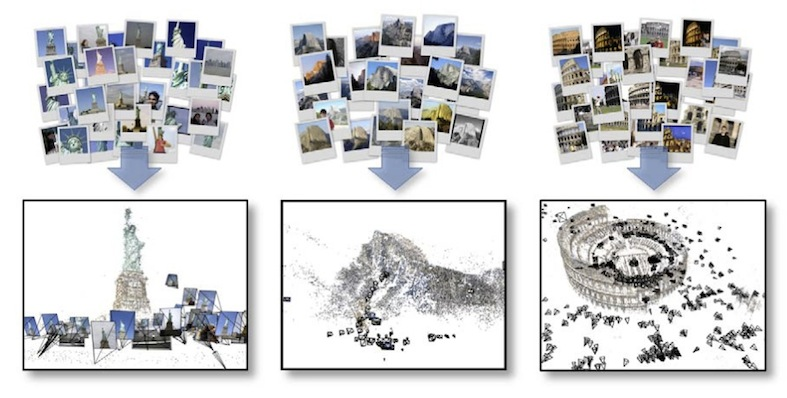
\includegraphics[width=0.95\textwidth]{image_synthesis.jpg}
\caption{3D mesh reconstructions from Internet photo collections, that typically can have dozens of millions of triangles \citep[][p.6]{Snavely2008}.}
\label{fig:image_synthesis}
\end{figure}\\
Still, as of lately, the research community does not emphasise on mesh decimation.
One of the reason for this, is the set of expectations that govern academic zeitgeist.
For example, ``good'' solutions are considered to be solutions that have been completely automated with little or none required input from the user.
However there is much to be gained and researched, once the user is seen as integral part of the process.
\begin{quote} \textit{``Decimation of generated models, often reduces the precision ... and while the generated meshes may have the correct level of detail, it is not represented in a structured form, usable in subsequent stages ... In many cases it would be more useful to rely on user input to generate a simplified, yet structured mesh that can be further manipulated.''} \citep[p.195]{Sylwan2011} \end{quote}
Bringing together the arguments of the last pages, the important question to ask now is, what kind of requirements should a modern mesh decimation algorithm focus on?

\section{Design Principles \& Workflow Regimes}
\label{introduction4}

The first step in deciding upon the design features of an application that simplifies meshes, is to acknowledge that there will never be one perfect solution to fit all possible scenarios.
Not only because there are always trade-offs to be made in engineering, but because there are conflicts of objectives that oppose each other diametrically.
For instance, it is not possible to ensure quasi 'Delaunay-Triangulation' in order to cater for the needs of an finite elements simulation and at the same time aggressively reduce the vertex count without loosing geometric detail\footnote{ Arguably it will be always a choice of just two out of the following three: good triangle shape / high decimation rates / optical fidelity -- and many other examples for such conflicts can be found.}.\\
 Instead, it shows more promise to put emphasis on a few selected, crucial aspects.
Thus our work focuses on two major principles that were decided beforehand:
\begin{itemize}
    \item Topological control of the decimation process.
    \item Artistic freedom by the means of user-guidance.
\end{itemize}
As for the first aspect -- topology control -- most algorithms can ensure the preservation of the topological genus of a given model\footnote{ With the notably exception of the class of vertex clustering algorithms, that by design, are agnostic to topological changes \citep[cf. the original paper by][]{Rossignac1993}.}, but normally topological features by themselves are not driving criteria for decimation.
Accounting for this poses some interesting research questions that have not yet been answered satisfactorily.
It is also the more theoretical and abstract part of the thesis.\\
The second aspect -- artistic freedom, i.e. user-guidance -- has some further ramifications that need to be pointed out.
Unquestionably it appears to be a good thing to give additional control to the user.
Not only can the hard problem of perceptual fidelity be handed over to the one instance best suited for the decision, but also there can be direct feedback incorporated to ensure the ideal outcome.
\begin{quote} \textit{``Often researchers are biased towards a fully automated solution or assume the user interaction needs to be targeted to a novice user.''} \citep[p.195]{Sylwan2011} \end{quote}
%Bild
\begin{floatingfigure}[r]{0.40\textwidth}
\centering
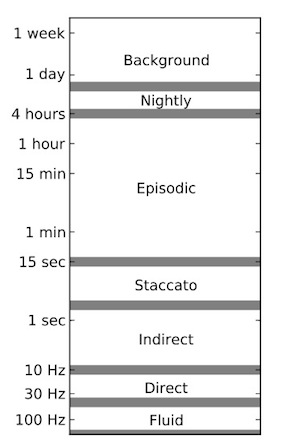
\includegraphics[width=0.30\textwidth]{workflow_regimes.jpg}
\caption{Response time to user input vs. workflow.}
\label{fig:workflow_regimes}
\end{floatingfigure}
Just adopting some measure of control not automatically yields better results. 
In order to leverage the outlined advantages, the entire system has to meet the needs of direct user interaction.
There is a balance between interaction and computation.\\
If a process gives perfectly accurate results automatically, it is a candidate to run unsupervised in an multiply hour offline scenario.
Whereas an algorithm that requires artist intervention, must run relatively quickly so artists get immediate feedback and iterate on it \citep[cf.][p.20]{Hillman2010}.
This sounds like an obvious observation, but research has shown, that missing certain levels of interactivity, ultimately decides upon how a tool is viewed as a whole and thereby determines the success and adoption rate of this technology \citep[cf.][]{Enderton2011}.
In summary, what we want is a very fast, hence smoothly interacting application that gives good results but invites the user to tweak any aspect of it until the best possible outcome is reached.
This is in short is what this thesis' goal is!
\begin{quote} \textit{``A workflow regime is defined as a range of system response times in which the artist’s relationship to the task is qualitatively similar ... technology is much more likely to succeed when it brings an artist’s workflow into a new regime ... we feel physically connected, albeit indirectly. This connection is critical for focused and rapid task achievement.''} \citep[p.2]{Enderton2011} \end{quote}

\section{The Outline of this Thesis}
\label{introduction5}

The introduction started with a general observations on trends:
The complexity from the point of view of Computer Graphics has increased dramatically over the last decades and is still on the rise.
This is especially true for geometric complexity, since even the best short-cuts suffer from undesired artifacts. 
With models getting more and more detailed, the need for good tools that can simplify meshes likewise increases. 
But instead of adding a new algorithm to the standard repertoire, we propose to focus on adopting techniques for user-guidance and topology control.
After this widely argument for our motivation, the rest of the thesis is structured pretty much straightforward.

The next section, chapter \ref{simplification0}, will very briefly discuss the historical development of the field of mesh decimation.
Not so much in order to give an exact overall account, but rather to give an overview of the principle techniques and the ideas behind them.
Bringing these ideas together we will try to formulate a taxonomy that structures the known approaches.\\ 
This is followed by chapter \ref{math0}, that functions as a primer for mathematical concepts which are crucial for the understanding and control of topology.
Retrieving correct topology information of a mesh and controlling it, is one of the key contributions of our work and although the comprehension of the involved mathematics is important, we try to not make it a mandatory prerequisite for the results section of the text.\\
Chapter \ref{topstoc0} finally details the contribution of our work in three sections.
Firstly some minor adaptions to the``TopStoc'' algorithm that we used as the foundation in section \ref{topstoc1}.
Then in \ref{topstoc2} we deal with the topological aspects, namely computing the precise Betti numbers for arbitrary meshes.
Finding all topological relevant features such as handles and tunnels, which is achieved by the means of gathering special groups of homologous edge loops.
And of course the ability to cut and delete parts of the mesh as well as mending boundaries.
Section \ref{topstoc3} finally describes the tools that give artistic freedom to the artist.
Among these are sketch tools to define resolution, point of view constraints for decimation plus visual feedback in form of Hausdorff visualizations and multiple instances of decimation results to easily make side-by-side comparisons.\\
The last part, chapter \ref{conclusion0}, then summarizes the work and gives an outlook on further research topics.
